\documentclass[12pt]{article}
\usepackage{setspace,graphicx,amsmath,geometry,fontspec,titlesec,soul,bm,subfigure}
\titleformat{\section}[block]{\LARGE\bfseries}{\arabic{section}}{1em}{}[]
\titleformat{\subsection}[block]{\Large\bfseries\mdseries}{\arabic{section}.\arabic{subsection}}{1em}{}[]
\titleformat{\subsubsection}[block]{\normalsize\bfseries}{\arabic{subsection}-\alph{subsubsection}}{1em}{}[]
\titleformat{\paragraph}[block]{\small\bfseries}{[\arabic{paragraph}]}{1em}{}[]
\setmainfont{Times New Roman}
\renewcommand{\baselinestretch}{1.15}
\renewcommand\contentsname{Inhaltverzeichnis}
\geometry{a4paper,left=2.5cm,right=2.5cm,top=2.5cm,bottom=2.5cm}
\begin{document}
	\newpagestyle{main}{            
		\sethead{}{Kapitel 6}{} 
		\setfoot{}{\thepage}{}
		\headrule
		\footrule
			}
	\pagestyle{main}
\tableofcontents
\newpage
\section{Tachymetrische Messungen}	
\subsection{Grundlagen und Systemübersicht}
Sensoren:
\begin{itemize}
	\item Horizontalrichtung
	\item Vertikalrichtung
	\item Distanz
	\item Neigung
	\item Grob- und Feinzielsuche
	\item Temperatur und Luftdruck
\end{itemize}
Aktoren:
\begin{itemize}
	\item Motoren
	\item Dioden(zu Zielsuche und Absteckung)
\end{itemize}
\subsection{Entfernungsmessung mittels Wave Form Digitizer (WFD)}
\subsection{Prüfung und Kalibrierung von Tachymetern}
\subsubsection{Tachymeterprüfung}
Eine Prüfung stellt fest, ob ein Gerät die Spezifikation einhält oder ob es geeinget ist, die Genauigkeitsanforderungen eine Anwendung zu erfüllen. \newline
\newline
Hierbei kann das ganze System oder einzelne Komponente überprüft werden \newline
\newline
Bei einer Kalibrierung wird der Unterschied zwischen Soll-Wert und Ist-Wert bestimmt. Dieser kann als Korrekturwert benutzt werden. \newline
\newline 
Eine Eichung ist eine Kalibrierung von Amtswegen(z.B geeichte Gewichte) \newline
\newline
FIG - International Federation of Surveys\newline
Leistungsüberprüfung / Vereinfachtes Testverfahren
\begin{itemize}
	\item Messung von 4 bekannten Strecken im vorgesehenen Arbeitsbereich (z.B 20 m bis 200 m)
	\item 3-malige Messung und Bestimmung des Mittelwertes
	\item Differenz zwischen Mittelwert und Soll-Wert muss kleiner als vorgegebene Grenzwert sein
	\item Analyse auf Maßstab und Nullpunktfehler möglich
\end{itemize}
Kalibrierähnliche Überprüfung / Vollständiges Testverfahren
\begin{itemize}
	\item Geradelinige Konfiguration mit 7 Punkten; Abstände im Arbeitsbereich
	\item Überprüfung der Spezifikation des Herstellers und der Signifikanz des Nullpunktfehlers
	\item Weiteres unter Kalibrierung
\end{itemize}
\subsubsection{Maßstab und Nullpunkt des EDM}
Instrumentelle Maßstab (Gerätmaßstab)\newline
Abweichung der Modulationsfrequenz (Messfrequenz) von der Sollfrequenz. \newline
\newline
Frequenzmessung des modulierten Infrarotlicht (für Phasenvergleichsverfahren) mittels eines temperaturstabilisierten Frequenzzählers:
\begin{itemize}
	\item direkter Abgriff
	\item indirekter Abgriff $\Rightarrow$ bei kontinuierlich abstrahlende EDM $\Rightarrow$ bei gepulst abstrahlenden EDM.
\end{itemize}
Frequenzkorrektur:
\begin{gather*}
	K_f = D_0 \frac{f_0 - f}{f} \\
\end{gather*}
$D_0$: gemessene Strecke, $f_0$: Soll-Frequenz, $f$: Ist-Frequenz. Frequenz zeigt (1) Einlauferlaten(bis zu 5 Minuten) und (2) und ist temperaturabhängig. \newline
\newline
Geräte mit internen Frequenzkorrektur: \newline
Temperaturabhängige Frequenz wird gespeichert und muss zum Vergleichen als $f_0$ genutzt werden.
\begin{gather*}
	f_0 = f_B + f_M \\
	f_M = A + B(t - t_0) + C(t - t_0)^2 + ......
\end{gather*}
mit $t_0$ Referenztemperatur und $t$ aktuelle Temperatur.  \newline
\newline
Beim Inpulsverfahren muss die Zeitbasis am Geräte gemessen werden (Drift der Uhr). Frequenz der Infrarotsignals ohne Bedeutung. \newline
\newline
Zuklischer Phasenfehler:\newline
Periodische auftretender Fehler mit der Periode $\frac{\lambda}{2}$, Entstehung durch elektrisches und optisches Übersprechen Bestimmung. Gleichmässige Verteilung von interferometrische gemessene Soll-Strecken über den Maßstab $\frac{\lambda}{2}$.
\begin{equation*}
	K_{zuk} = A \cdot (2\pi \cdot \frac{D_i - C}{\frac{\lambda}{2}})
\end{equation*}
$A$: Amplitude, $C$: Phasenlage, $D_i$: Strecke im Feinmaßlage. $A$ und $C$ können durch Ausgleichung geschätzt werden. \newline
\newline
Nullpunktfehler Additionskonstante, $\Rightarrow$ Kombination aus EDM und Prismenanteil Kalibrierung. 
\paragraph{Eindeutige Lösng}
\begin{gather*}
	D_{12} = D_{12,gem} + K_0 \\
	D_{23} = D_{23,gem} + K_0 \\
	D_{13} = D_{13,gem} + K_0 \\
	D_{13} = D_{12} + D_{23} \\
	D_{13,gem} + K_0 = D_{12,gem} + K_0 + D_{23,gem} + K_0 \\
	D_{13,gem} - D_{12,gem} - D_6{23,gem} = K_0 \\
\end{gather*}
\paragraph{Überstimmete Lösung}
\begin{itemize}
	\item Messung von Strecken in allen Kombinationen
	\item Ausgleichung zu Bestimmung des Nullpunktfehlers
	\item Frequenzkorrektur vorab anbringen
	\item Strecken müssen nicht bekannt sein
	\item im Vergleich zu Eindeutige Lösung verbesserte Genauigkeit und zuverlässigkeit
	\item zyklischen Fehler vorab bestimmen und Korrigieren
\end{itemize}
\subsubsection{Teilkreiskalibrierung}
Abweichungen der IST-teilungsintervall von den Soll-Intervall (z.B 1 gon); existieren zuklische und zufällige Abweichungen Bestimmung der Differenzen durch interferometrische Winkelmessung in Produktionsprozess. 
\subsection{}
\subsubsection{Automatische Zielerfassung und verfolgerung}
Ziel:
\begin{itemize}
	\item Tachymeter kann Ziele selbständig messen und verfolgen.
	\item 1-Person Station (zu schaffen)
	\item Möglichkeit kinematische Messungen
\end{itemize}
Voraussetzung:
\begin{itemize}
	\item Motorisierung des Tachameters
	\item Ziel muss mit Reflektor signalisiert sein
	\item zusätzliche Sensoren
	\item kommunikation zwischen Tachymeter und Reflektor / Bedieneinheit
\end{itemize}
Nebeneffekt:
\begin{itemize}
	\item Benutzerabhängsger Einstellfehler eliminiert
\end{itemize}
\subsubsection{Grobzielsuche}
\begin{itemize}
	\item Auffinden der Zielpunkte im Objektraum, möglichst ohne Vorinformation
	\item Abschluss, wenn Reflektor im Gesichtsfeld des Tachymeterfernrohrs
\end{itemize}
Verschiedene Variante: \newline
Passiver Reflektor
\paragraph{Passiver Reflektor}
\subparagraph{(1)}
spezielle (ensoren ur Grobzielsuche, Reflektion von Reflektor wird am Gerätdetektiert(z.B Leica Point Search))
\begin{itemize}
	\item 40 gon aufgefächerte Laserebene(vertikal)
	\item HZ - Drehung des Instruments
	\item Reflektiertes Signal legt Hz-Winkel auf 50 mgon fest
	\item V-Kippung mit gebündelten Signal
	\item V-Winkel auf 50 mgon
\end{itemize}
\subparagraph{(2)}
Wie (1) aber Ausfächerung nur auf $10''$
\begin{itemize}
	\item Scannen in mehren Durchläufen mit unterschiedlichen V-Winkel (z.B Treimble, Topcon/historisch)
\end{itemize}
\paragraph{Aktiver Reflektor}
\subparagraph{(3)}
wie (1), aber Reflektor sendet aufgefächertes Signal (67gon V $\times$ 220gon Hz) an das Instrument, von den Reflektor eindeutig zu identifizieren(Trimble, Topcon).
\subparagraph{(4)}
Reflektor mit Messeinrichtung. (Geodimeter 4000, historisch)
\begin{itemize}
	\item Reflektor wird auf Tachymeter ausgerichtet
	\item gemessener Vertikalwinkel wird an Tachymeter übermittelt
	\item abschließende Hz-Drehung liegt zweiten Winkel fest 
\end{itemize}
\subparagraph{(5)}
Reflektor ist mit GNSS-Empfänge ausgerüstet(Low Cost) Ausrichtung des Tachymeters mittels Koordinaten von Tachymeter und Prisma (Trimble, Topcon)
\paragraph{Ziel-Identifikation}
bei (3) bis (5) ohne Probleme \newline
bei (1): gefächerter Scan mit und ohne Zielprisma, Differenz zeigt zu identifizierendes Prisma.
\subsubsection{Feinzielsuche}
Bestimmung der Ablage zwischen Fadenkreuz und Reflektormitte\newline
Voraussetzung: Reflektor im Gesichtsfeld durch Grobzielsuche oder manuellen Anzielen. \newline
2 Verfahren:
\subparagraph{(a) Bildverarbeitung}
(passive Reflektor, Leica, Topcon)
\begin{itemize}
	\item Detektion des reflektierten Lichts durch CCD oder CMOS-Array
	\item Bestimmung der Reflektormirte durch Schwerpunktbildung $(x', y')$
	\item Transformationsparameter $x',y'$ nach $\Delta HZ$, $\Delta V$ bekannt.
\end{itemize}
	Ablagen $\Delta Hz$ und $\Delta V$ bestimmt.
\subparagraph{(b) Quadratendetektor}
(aktiver Reflektor, Trimbel)
\begin{itemize}
	\item Detektion des ausgesanten Signals mittels Quadratendetektor oder Poppelquadratendetektor.
	\item Bestimmung der Reflektormitte durch lineare Funktion der Intensitäten der 4 Quadraten (Bedienung, in jedem Quadraten Licht)
	\item Transformation wie unter (a)
\end{itemize}
Unterschiedliche Gesichtsfelder
\subparagraph{(1) ATR $\neq$ Fernrohr}
\begin{itemize}
	\item Punkte am Rand nicht mit ATR messbar
	\item spiralförmige Suche bis ATR messen kann
	\item Alternative: GNSS-Suche
\end{itemize}
\subparagraph{ATR $\neq$ EDM}
\begin{itemize}
	\item Streckenmessung nicht möglich
	\item Neuausrichtung des Fernrohrs (Verklenerung von $\Delta Hz$ und $\Delta V$)
\end{itemize}
\subsubsection{Verfolgung eines bewegten Ziels}
$\Longrightarrow$ Verfolgung eines Reflektors im Stop-and-go-Moduls \newline
Regelkreis mit Feinzielsuche und Motoren:
\begin{figure*}[ht]\centering
	\subfigure[]{
		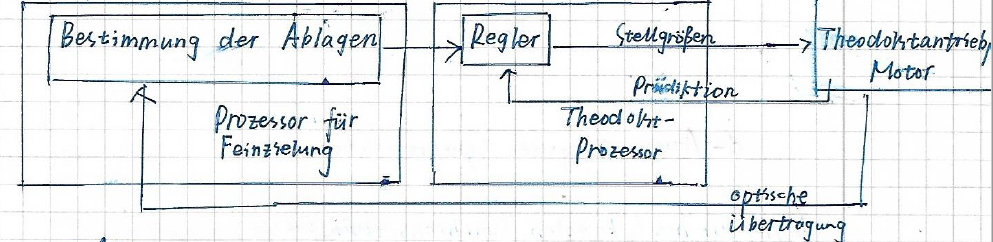
\includegraphics[width=0.9\textwidth]{flussdiagramm.png}}
\end{figure*}
\begin{itemize}
	\item Ablage nach 7.1-c berechnet
	\item Regler berechnet Stellgräßen für Motoren, um Ablagen wegzustellen
	\item Zielverlust führt zur Unterbrechung der Ablagenbestimmung
	\begin{itemize}
		\item Stellgräßen aus Bewegungsmodell für einige Sekunden (unveränderte Geschwindigkeit und Bewegungsrichtung)
		\item danach: Grobzielsuche, Spiralsuche, GNSS-Suche
	\end{itemize}
\end{itemize}
\subsubsection{Kinematische Positionsbestimmung}
\begin{itemize}
	\item Positionsbestimmung eines bewegten Reflektors
	\item Reglung zur Verfolgung wie in 7.4-d
	\item Zusätzliche Streckenmessung im Tracking mode
	\item Messrage: Trimble: 20Hz, Leica: 8Hz
\end{itemize}
Abschätzung maximaler Positionsfehler: \newline
\begin{table}[ht] \centering
	\begin{tabular}{|l|l|l|}
		\hline
		$\Delta t$ & $v = 3km/h$ & $v=50km/h$ \\ \hline
		0,15s      & 12,5cm      & 2,1m       \\ \hline
		1ms        & 0,8mm       & 1,4cm      \\ \hline
	\end{tabular}
\end{table}
Messanordnung zur Synchroniseitionsfehlerbestimmung \newline
\begin{figure*}[ht]\centering
	\subfigure[Auswirkung des Synchronisationsfehlers]{
		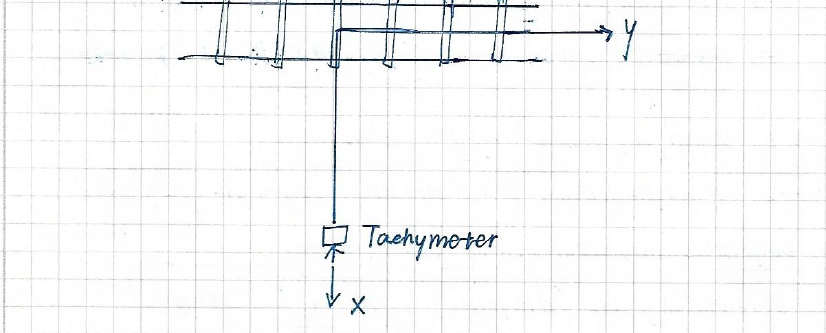
\includegraphics[width=0.6\textwidth]{bild.png}}
\end{figure*}
Korrektur bei bekannten Synchronisationsfehler: \newline
Trajektorienelemente:
\begin{gather*}
	t_f = \arctan \frac{\Delta x}{\Delta_y} \\
	z_f = \arccos \frac{s_f}{\Delta_H} \\
	s_f = \sqrt{\Delta x^2 + \Delta y^2 + \Delta z^2} = v \cdot \Delta t \\
\end{gather*} 
$v$, $\Delta t$ sind bekannt, $\Delta x$, $\Delta y$, $\Delta H$ aus Vorepochen \newline
gemessene Koordinaten, verfälscht
\begin{gather*}
	x_{R'} = x_s + s_D \cdot \sin z_R \cos t_R \\
	y_{R'} = y_s + s_D \cdot \sin z_R \sin t_R \\
	H_{R'} = H_s + s_D \cos z_R
\end{gather*}
Bestimmung von $s_R$
\begin{gather*}
	s_D^2 = s_R^2 + s_F^2 - 2 \cdot s_R \cdot \cos \alpha \\
	\Rightarrow s_R = s_F \cos \alpha \pm \sqrt{s_D^2 - s_F (1 - \cos^2\alpha)}
\end{gather*}
\begin{itemize}
	\item $\theta$ ohne Bedeutung
	\item $s_D \gg s_F$
\end{itemize}
\begin{gather*}
	\Longrightarrow s_R = s_F \cos \alpha + s_D - \frac{1}{2} \frac{s_F^2}{s_D^2} (1 - \cos^2 \alpha)
\end{gather*}
Bestimmung von $\alpha$: \newline
Seitenkosinussatz des sphärischen Trigonometrie
\begin{equation*}
	\cos \alpha = \cos z_F \cos z_R + \sin z_F \sin z_R  \cos (|t_F - t_R|)
\end{equation*}
Korrekte Koordinaten:
\begin{gather*}
	x_R = x_s + s_R \cdot \sin z_R \cdot \cos t_R \\
	y_R = y_s + s_R \cdot \sin z_R \cdot \sin t_R \\
	H_R = H_s + s_R \cdot \cos z_R
\end{gather*}
\subsection{Reflektorlose Entfernungsmessung}
\begin{itemize}
	\item höhere Intensität des Sendesignals (Strecke)
	\item Messsignal wird vom Objekt reflektiert, nicht vom Reflektor
	\item Reichwert: $\leq 2km$
	\item Typische Genauigkeit: $3mm + 3ppm$
	\item Koaxiale Anordnung besetzt höchste Genauigkeit 
	\item Problem der Punkt: identifikation
	\item Genauigkeit wird folgelich auch von Oberflächen beschaffenheit und Auftrittwinkel beeinflust
	\item starke Parallelstät zum Laserscanning
\end{itemize}
\end{document}
